\section{Introduction}
\begin{figure}[htbp]
\centering
\makebox[\linewidth][c]{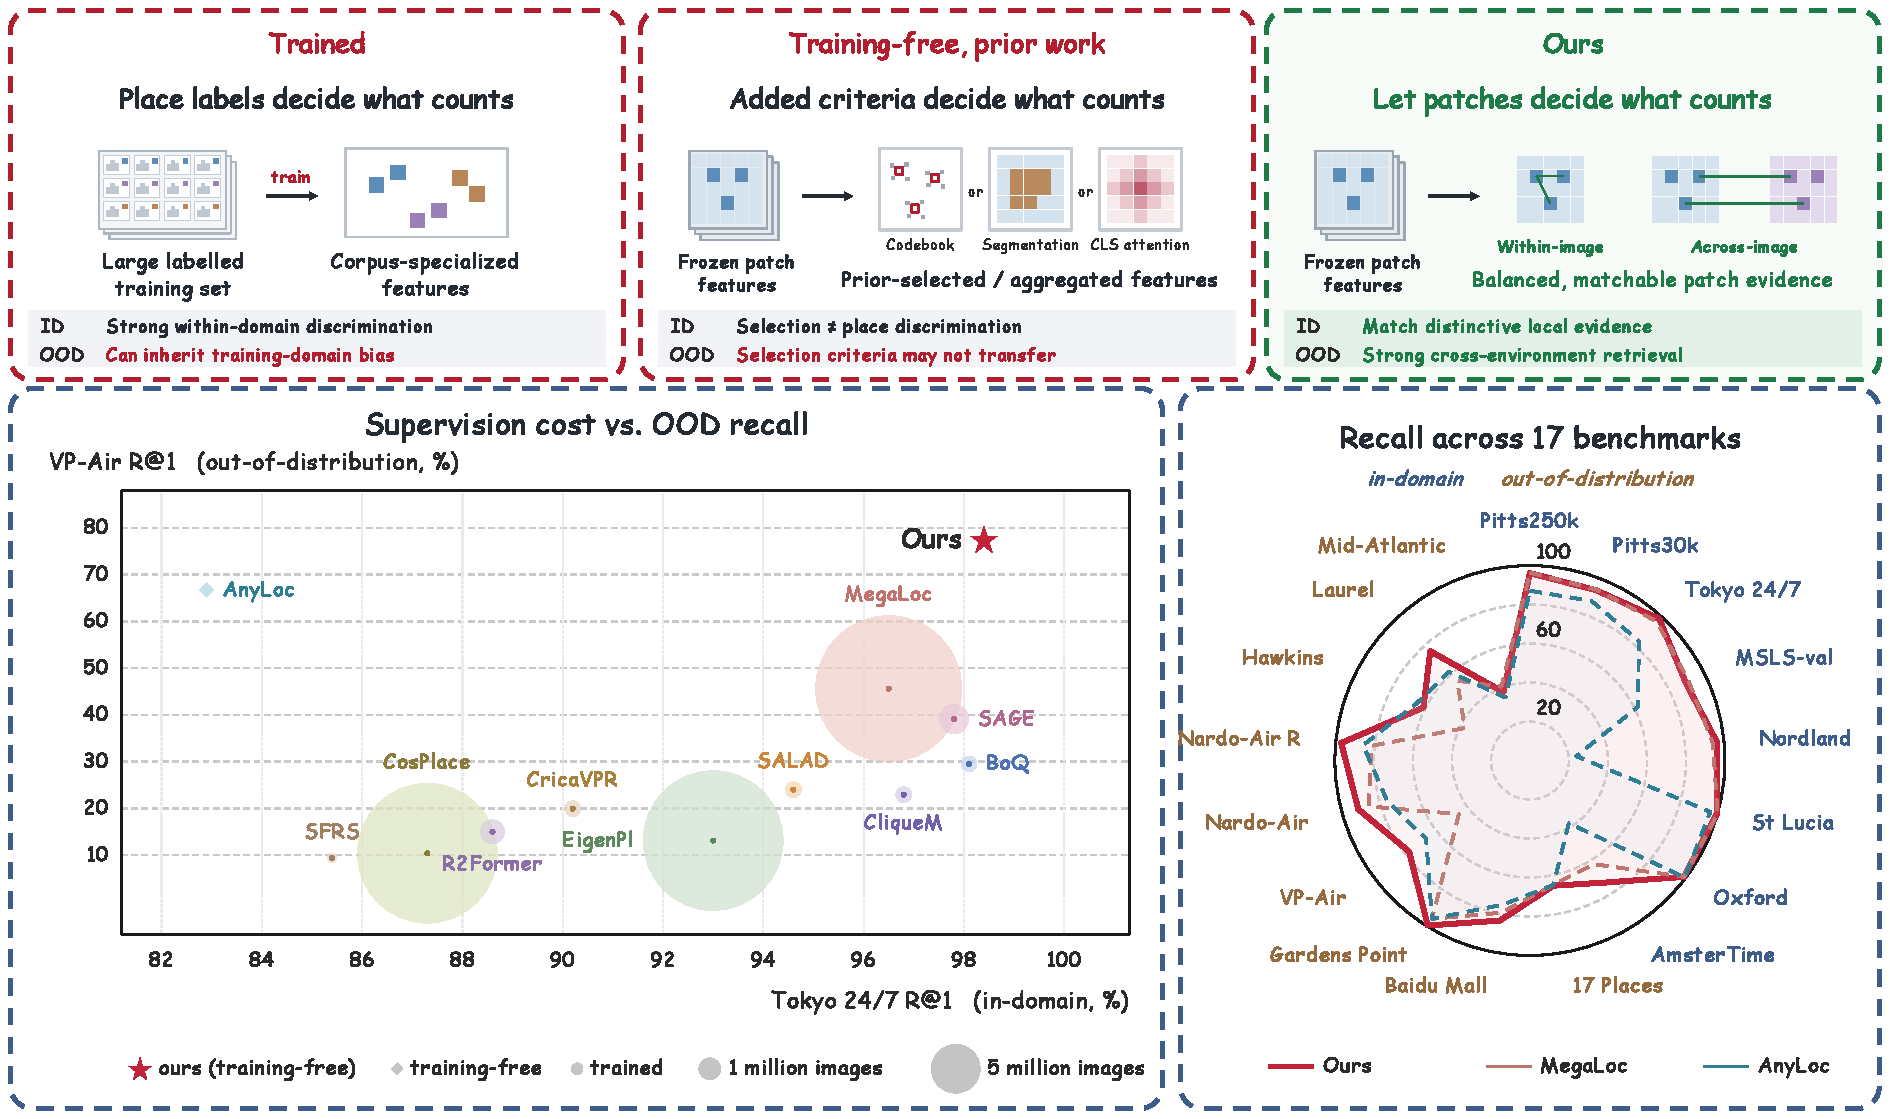
\includegraphics[width=\linewidth]{figures/teaser_v6.pdf}}
% \caption{\textbf{Three ways of deciding what an image contributes.} \textbf{A}: a representation shaped by place-labelled supervision. \textbf{B}: patches selected or aggregated by a criterion fixed outside the pair of images. \textbf{C}: ours, where both decisions are read from patch-to-patch similarities inside the pair. \textbf{D}: mean R@1 on the 8 standard benchmarks against the 9 cross-environment ones, with marker size increasing with the number of labelled training images; SFRS is omitted, its standard mean falling far below the range shown. \textbf{E}: R@1 on all 17 benchmarks.
\caption{\textcolor{red}{\textbf{Overview and performance (R@1).} (A) Trained methods require large-scale labelled datasets, limiting their generalisation to cross-environment settings. (B) Prior training-free methods avoid this training cost and generalise better, but suffer a performance drop on standard VPR benchmarks. (C) Our training-free method instead applies frozen patch features directly, using patch similarity both within and across images for retrieval. (D) Training cost versus performance of our method and baselines on 17 benchmarks, averaged separately across standard and cross-environment VPR benchmarks. (E) Performance of the proposed method against the state-of-the-art trained and training-free baselines.}}
\label{fig:teaser}
\end{figure}
% Visual Place Recognition (VPR), also known as visual geo-localization, is a fundamental task in computer vision that aims to determine where a photograph was taken by matching it against a database of geo-tagged images. It underpins loop closure in visual SLAM, re-localization for autonomous driving where satellite positioning is unreliable, and city-scale mapping services that anchor imagery to a map, and increasingly it is asked to work where no street-view corpus exists: aerial and drone navigation, inspection robots in mines, caves and tunnels, indoor delivery and service robots, underwater vehicles surveying the sea floor, and the matching of historical photographs to the present day. The databases involved range from a few hundred images in an indoor survey to tens of millions across a city, so a practical system has to stay accurate as the imagery, the environment and the scale of the map change.

Visual Place Recognition (VPR) is a long-standing computer vision challenge that aims to recognise where a query image was captured by matching it to a database of images tagged with their locations. VPR is essential to many core applications, such as visual SLAM, re-localisation in autonomous driving, and city-scale mapping services. Classical and standard VPR benchmarks mainly target this setting, using largely standard street-view images. However, we notice that VPR is increasingly required in a broader range of scenarios~\citep{anyloc}, such as aerial and drone navigation, indoor delivery and service robots, underwater vehicles surveying the sea floor, and the matching of historical photographs to present-day scenes. We refer to these scenarios and their corresponding benchmarks as cross-environment benchmarks. In this paper, we argue that advanced VPR solutions should generalise not only to standard VPR benchmarks but also to cross-environment benchmarks.

% Existing approaches fall into two families. The dominant family learns a representation from place labels. NetVLAD \citep{netvlad} makes soft assignment to a codebook differentiable and trains it under weak supervision, and later work follows this template through classification over geographic cells \citep{cosplace,eigenplaces}, curated labels at scale \citep{gsvcities}, feed-forward pooling \citep{mixvpr}, and aggregation over frozen DINOv2 \citep{dinov2} tokens with optimal transport \citep{salad}, learned queries \citep{boq} or adapters \citep{selavpr}. The accuracy of these methods is bought with annotation: GSV-Cities \citep{gsvcities} provides about half a million street-level images over sixty thousand labelled places, the SF-XL line \citep{cosplace,eigenplaces} trains on more than forty million, and recent systems combine several such corpora or tune the backbone itself under parameter-efficient schemes \citep{megaloc,sage}. The second family removes the annotation and reads a frozen foundation model directly, aggregating patch tokens against a fitted vocabulary \citep{anyloc}, over segmentation proposals \citep{segvlad}, or at keypoints selected by class-token attention \citep{effovpr}.

Existing VPR methods are mainly training-based approaches, which require a large amount of annotated data for training. Classical methods such as NetVLAD~\citep{netvlad} make soft assignment to a codebook differentiable and train it under weak supervision, while later work follows this template through classification over geographic cells~\citep{cosplace,eigenplaces}, curated labels at scale~\citep{gsvcities}, or feed-forward pooling~\citep{mixvpr}, among others. Recent advanced methods achieve large performance improvements, but these gains are largely driven by increasingly large-scale annotated training sets: for example, GSV-Cities~\citep{gsvcities} provides about half a million street-level images over sixty thousand labelled places, while the SF-XL dataset~\citep{cosplace,eigenplaces} contains more than forty million annotated samples. Recent state-of-the-art methods, such as~\citep{megaloc}, gather even more annotated samples to train their models, achieving the best results but relying heavily on the scale of the annotated training set, as shown in Figure~\ref{fig:teaser}D. Even with millions of annotated samples, however, these state-of-the-art methods tend to learn environment- or domain-specific features that do not generalise well as shown in Figure~\ref{fig:teaser}A), suffering a performance drop on cross-environment benchmarks, as shown in Figure~\ref{fig:teaser}D\&E. 
% Recent training-free VPR methods~\citep{anyloc} remove the large scale annotation dependency and utilize a frozen large vision model directly with some post processing which  against a fitted vocabulary \citep{anyloc}, over segmentation proposals \citep{segvlad}, or at keypoints selected by class-token attention \citep{effovpr}.


To address this data-dependency challenge, training-free VPR methods have recently been proposed~\citep{anyloc,effovpr}, which aim to exploit the generalisation ability of large vision models, such as DINO backbones~\citep{dinov2} or SAM~\citep{kirillov2023segment}, to better solve VPR across a wide range of environments. These methods often generalise better than trained methods in the cross-environment setting, but fail on standard VPR benchmarks, as shown in Figure~\ref{fig:teaser}D-E. We argue that current training-free methods, which apply various strategies to obtain prior-selected features (Figure~\ref{fig:teaser}B), do not fully utilise the potential of these large vision models.
% However, both families decide what an image contributes using information from outside the pair of images being compared, and Figure~\ref{fig:teaser} illustrates the cost. The first cell of the top row depicts the supervised recipe, in which an image is related to a labelled corpus. The learned features therefore inherit the imagery that corpus contains, and the scatter plot below makes the consequence explicit: every trained method sits high on the standard axis and low on the cross-environment one, while the marker area records the millions of labels it consumed. The second cell depicts the training-free recipe, in which a patch is related to a criterion fixed elsewhere, such as an attention map trained to locate objects in web photographs, a codebook estimated on another collection, or a segmenter's notion of an object. None of these criteria was designed to answer which parts of a scene identify a place. The two questions differ: a single window in a facade of identical windows is locally salient and is retained, yet it cannot distinguish this building from its neighbour, whereas a plain strip of pavement that appears once may be the only distinctive content in the frame. On street-view imagery the two answers coincide often enough that the substitution is harmless. Away from street view they diverge, and the training-free method that selects patches by attention loses $11.6$ mean R@1 between the two blocks (Table~\ref{tab:breadth}). This is why training-free methods, despite requiring no data, still trail supervised ones in accuracy.

% To address these issues, we propose \method{}, a training-free VPR pipeline that keeps the decision inside the pair of images being compared, as shown in the third cell of Figure~\ref{fig:teaser}. \method{} reads two tables of patch similarity from a single frozen forward pass. Within an image, its self-similarity is thresholded and summed along each row, which counts how many of the image's own patches resemble a given one; the reciprocal of this count is the distinctiveness of that patch, and it solves a classical democratic-aggregation condition when repeated content forms blocks of near-duplicates. Between two images, the cross-similarity table is reduced in two ways: a bilinear contraction that factorizes into one descriptor per image and scans the database, and a row-wise maximum that does not factorize and fine-ranks a shortlist. Extensive experiments on seventeen benchmarks, under a single configuration held fixed throughout, show that \method{} achieves $93.2$ mean Recall@$1$ on eight standard VPR benchmarks and $76.6$ on nine cross-environment benchmarks spanning degraded, subterranean, indoor, aerial and underwater imagery, compared with $65.1$ for the strongest supervised method on the latter.

\textcolor{red}{To address these challenges, we propose \method{} (Unified Patch Similarity), a simple and effective training-free method for VPR. \method{} first partitions the input images, whether queries or database images, into patches. A frozen vision model is then applied to extract patch features. These patch features are then applied in a series of patch similarity computations, in different forms, for patch importance, coarse ranking, and final reranking, with more details in Section~\ref{sec:method}. We summarise our contributions as follows:}

% \textcolor{red}{
% \noindent Our contributions are summarized as follows:
\begin{itemize}[leftmargin=*,itemsep=1pt,topsep=3pt]
% \item \textcolor{blue}{We remove the reliance of VPR on annotated data and propose \method{}, a simple and effective training-free pipeline.}
% \item \textcolor{blue}{We derive a training-free, image-adaptive patch weighting scheme from within-image self-similarity, suppressing repetitive visual patterns without place-specific supervision.}
% \item \textcolor{blue}{We reuse the same patch interaction space across both retrieval stages: its pooled second-order statistics provide a compact coarse representation, while its row-wise maxima provide fine-grained candidate-specific matching.}
% \item We achieve strong results on street-level imagery and beyond it under one fixed configuration, reaching $93.2$ mean Recall@$1$ on eight standard VPR benchmarks, on par with supervised systems trained on tens of millions of labels, and $76.6$ on nine cross-environment benchmarks where the strongest of those systems attains $65.1$. As a plug-in module, our second-stage rule further improves ten existing pipelines, by $+5.6$ and $+9.7$ R@1 when it replaces an existing fine-ranker and by $+9.1$ to $+17.8$ when it is added to a single-stage method.
\item  We remove the reliance of VPR on annotated data and propose \method{}, a training-free pipeline. It only requires a feature extractor for patch features, followed by a series of patch-similarity computations for VPR.   
\item We conduct a comprehensive evaluation on 17 benchmarks, on which the proposed \method{} achieves state-of-the-art results 
% \item We achieve strong results on street-level imagery and beyond it under one fixed configuration, reaching $93.2$ mean Recall@$1$ on eight standard VPR benchmarks, on par with supervised systems trained on tens of millions of labels, and $76.6$ on nine cross-environment benchmarks where the strongest of those systems attains $65.1$. As a plug-in module, our second-stage rule further improves ten existing pipelines, by $+5.6$ and $+9.7$ R@1 when it replaces an existing fine-ranker and by $+9.1$ to $+17.8$ when it is added to a single-stage method.
\end{itemize}
% }